\chapter{Einleitung}\label{ch:einleitung}
\glqq I recently predicted the last mainframe will be unplugged on March 15, 1996\grqq\footnote{\cite{Alsop.1993}} - ein in der Großrechner-Welt bekannt gewordenes Zitat.
Es handelt sich um eine 1993 getroffene Vorhersage, nämlich dass der letzte Mainframe, auch Großrechner genannt, am 15 März 1996 abgeschaltet werden würde.
Warum war diese Vorhersage falsch? 
Wieso wird sich im Jahre 2020 immer noch mit dieser Technologie beschäftigt? 
Und was genau ist ein Großrechner?

Kurz gesagt ist ein Großrechner\footnote{Beschreibung im Absatz \ref{sec:mainframe} zu finden} ein leistungsstarkes, zentralisiertes Serversystem.
In dieser Arbeit wird nur auf Mainframes aus dem Hause IBM, die sogenannte z-Plattform, eingegangen.
Damit ist auch der Technologiestack festgelegt.
Das verwendete Betriebssystem ist z/OS, darauf werden Middleware Produkte wie CICS\footnote{Anwendungsserver, CICS Beschreibung Absatz \ref{cics}}, das Datenbanksystem Db2\footnote{ Beschreibung Absatz \ref{sssec:db2}} sowie die Messaging Lösung \glqq IBM MQ\grqq{}\footnote{Beschreibung im Absatz \ref{sec:mq} zu finden} betrieben.
Als Programmiersprachen werden z.B. COBOL, IBM Assembler, C und C++ verwendet. 
Seit ca. 1997 ist auch Java auf dem Mainframe verfügbar. \footnote{\cite{Steegmans.2003}}.

Der IBM Mainframe hat eine lange Geschichte.
Vor mehr als fünfzig Jahren wurde der erste Großrechner, das sog. \glqq System/360\grqq{} vorgestellt.
Bis in die 90er Jahre spielte der IBM Mainframe eine Hauptrolle auf dem Computermarkt, dann gewannen zunehmend verteilte Client-Server-Systeme an Bedeutung.\footnote{\cite{Ceruzzi.2003}}
Seitdem gilt der Mainframe bereits als \glqq  legacy\grqq{} und damit als \glqq Altlast\grqq\footnote{\cite{.22.2.2020}}.

Wieso also wird sich mit der Mainframe Technologie noch beschäftigt? Eine Antwort: Auf dem Mainframe werden auch im Jahr 2020 geschäftskritische Anwendungen in der ganzen Welt gehostet.
So verwenden laut IBM 92 der 100 weltweit führenden Banken für ihre Kernabläufe einen IBM Mainframe.
Dies beinhaltet 87 Prozent aller Kreditkartentransaktionen und ca. 350.000 Transaktionen pro Sekunde.\footnote{\cite{.25.2.2020c}}
Inklusive dieser Transaktionen verarbeiten Großrechner heutzutage weltweit circa 1,2 Millionen CICS Transaktionen pro Sekunde.\footnote{\cite{.23.11.2019b}}
Im Vergleich hierzu werden 63.000 Google Suchanfragen pro Sekunde abgesetzt.  \footnote{\cite{.02.12.2019}}

Aus der Kombination von hohem Workload, der Abhängigkeit von einem Hersteller (IBM) und dem als veraltet geltenden Technologiestack entstehen jedoch zunehmend Risiken.
Es wird immer schwieriger, Nachwuchs in diesem Bereich zu finden.
Zum einem, da Mainframe-Know How kaum noch an Universitäten gelehrt wird.
Die Seite des Hochschulkompass\footnote{\cite{.09.02.2020}} liefert z.B. weder für \glqq Mainframe\grqq{} noch für \glqq Großrechner\grqq{} einen Treffer.
Zum anderen ist der demographische Faktor bei den Wissensträgern nicht zu vernachlässigen. Diese sind - wie die Technologien auf dem Mainframe - in die Jahre gekommen und erreichen das Rentenalter.\footnote{\cite{.25.2.2020f}}

Ein weiteres Problem ist, dass eine Firma, die einen IBM Großrechner mit z/OS betreibt, von dem oben genannten proprietären Technologiestack abhängig ist, dass heißt, es existiert eine starke Hersteller- und Plattformabhängigkeit, z.B. in Bezug auf CICS, Db2, IBM-COBOL-Compiler, IBM Assembler.

Offensichtlich betreiben dennoch etliche Firmen einen IBM Großrechner.
Dazu zählen hauptsächlich Banken, Versicherungen, Fluggesellschaften usw.\footnote{\cite{.25.2.2020c}}
Der gemeinsame Nenner dieser Unternehmen ist, dass sich über die Jahre und Jahrzehnte enorme Investitionen auf dem Mainframe angesammelt haben.
Die entstandenen, hochgradig geschäftskritischen Kernsysteme haben hohe Anforderungen an Massendatenverarbeitung, Sicherheitsstandards und Hochverfügbarkeit.
All diese Punkte sprechen nach wie vor für die Nutzung eines Großrechners, z.B. auch bei der DATEV e.G. (Kommentar: hier wäre ein Zitat schön, von einer Bank o.ä. ich schau mal ob ich was finde)

Die DATEV e.G. wurde am 14.02.1966 von 65 Steuerbevollmächtigen gegründet.
Sie verfolgten mit der Gründung das Ziel, Buchführungsaufgaben für ihre Mandanten mit Hilfe der neu aufkommenden EDV zu bewältigen.
Aufgrund hohen Mitgliederwachstums wurde hierfür bereits 1969 in einen firmeneigenen IBM-Großrechner investiert.\cite{.25.11.2019c}
Heute umfasst das Leistungsspektrum der DATEV e.G. unter anderem das Rechnungswesen, Personalwirtschaft, Consulting, IT-Sicherheit, Weiterbildung für ihre Kunden, in erster Linie Steuerberater, Wirtschaftsprüfer und Rechtsanwälte, und deren Mandanten.
Ein nicht unbeträchtlicher Teil dieser betriebswirtschaftlichen Anwendungen läuft bis heute ganz oder als Backend von Client-Anwendungen auf einem IBM Großrechner im DATEV Rechenzentrum.
So werden pro Tag circa 150.000 Batch Jobs\footnote{Beschreibung in Absatz \ref{ssec:job}} und circa 90 Millionen CICS-Transaktionen verarbeitet.
Diese Last wird von circa 14.000 aktiven Modulen erzeugt.
Wie in der Abbildung \ref{fig:Programmiersprachen} zu sehen ist, ist COBOL mit circa 46\% Prozent die am häufigsten verwendete Programmiersprache am Großrechner bei der DATEV e.G..
Durch diese Module werden unter anderem im Monat circa 11 Millionen Lohnabrechnungen erstellt und circa eine Millionen Umsatzsteuer-Voranmeldungen durchgeführt. 
2018 wurde mit den DATEV Produkten erstmals die Umsatz-Milliarde erreicht.\footnote{\cite{.27.2.2020b}}

\begin{figure}
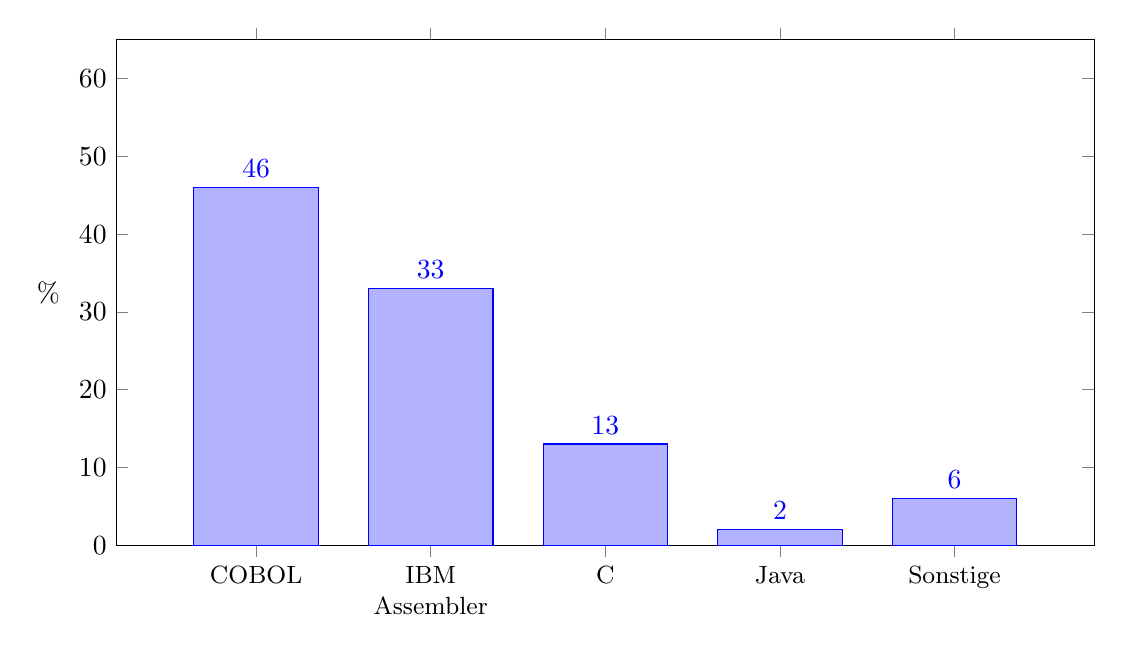
\begin{tikzpicture}
\begin{axis}[
             width=14cm,
             height=8cm,
             symbolic x coords={COBOL,IBM Assembler,C,Java, Sonstige},
             x tick label style={font=\small,text width=1.7cm,align=center},
             xtick=data,
             nodes near coords,
      	  nodes near coords align={vertical}, 
             ymin=0,
             ymax=65,
             ylabel=\%,
             ylabel style={rotate=-90},
             ybar,
             enlarge x limits=.2,
             bar width=45pt,
             ]
\addplot coordinates{(COBOL,46) (IBM Assembler,33) (C,13) (Java,2) (Sonstige,6)};
\end{axis}
\end{tikzpicture}
\centering
\caption{Anteil der verwendeten Programmiersprachen auf dem Mainframe bei DATEV eG in Prozent}
\label{fig:Programmiersprachen}
\end{figure}

\section{Problemstellung}\label{sec:probstell}
Im Jahre 2020 ist der größte Konkurrent für den Mainframe die Cloud.
Laut einer Vorhersage aus dem Jahr 2018\footnote{Statistik im Anhang \ref{app:itworkload}} soll im Jahre 2020 circa 79 Prozent des weltweiten Workloads in einer Cloud verarbeitet werden.
Für die Entwicklung von neuen Online-Anwendungen im cloud-native Stil wurde bei der DATEV e.G. eine Platform-as-a-Service (PaaS)-Lösung geschaffen und neue DevOps\footnote{Siehe Absatz \ref{sec:analysecloud}} Prozesse aufgebaut.
Dies ist im Cloud-Zeitalter nötig, um mit einer verbesserten Entwicklungseffizienz und neuen Architekturen Anwendungen (\glqq Apps\grqq) schneller auf den Markt bringen und auf Kundenanforderungen schneller reagieren zu können. Stichwort: Continuous Integration, Continuous Delivery (CI/CD)\footnote{Siehe Absatz \ref{sec:cicd}}.
Ein Baustein der effizientern Prozesse durch PaaS sind die sog. \glqq Self Services\grqq.
D.h., Entwicklerteams können sich über sog. \glqq Cloud Services\grqq, z.B. Datenbanken wie PostgreSQL, Mongo und Messaginglösungen wie Kafka entweder manuell über einen Marktplatz (siehe Abbildung \ref{fig:markt}) oder automatisiert per \glqq Build-Pipeline\grqq{} eine  Laufzeitumgebung für ihre Anwendung zusammenbauen.
Eine genaue Beschreibung der Begrifflichkeiten erfolgt im Absatz \ref{sec:cloudnative}.
Den Entwicklern steht, neben modernen Entwicklungsumgebungen (IDE\footnote{Integrated Development Environment wie IntelliJ oder Eclipse}) und einer Sourceverwaltung mit Git, auch eine sog. \glqq Toolchain\grqq{} zur Verfügung. Diese beinhaltet Tools für Build, Test, Quality Gates und Deployment. 
Damit wird der Entwicklungsprozess automatisiert und man erhofft sich eine hohe Entwicklereffizienz. (Kommentar: hier würde ich nach wie vor die Grafik von unserem go/cloud Sharepoint mit einbinden)

Der Entwicklungsprozess für z/OS Anwendungen bei DATEV e.G. erscheint im Vergleich zu dieser PaaS-Lösung veraltet.
So wurde 2010 eine auf Eclipse basierende Entwicklungsumgebung für COBOL und IBM Assembler in der DATEV e.G. flächendeckend bereitgestellt.
Zuvor - und teilweise heute noch -  wurde mit Hilfe der in Abbildung \ref{fig:3270} gezeigten Oberfläche, dem sog. ISPF gearbeitet.
Diese stellte z.B. nur ein Syntaxhighlighting zur Verfügung.
\begin{figure}[h]
\centering
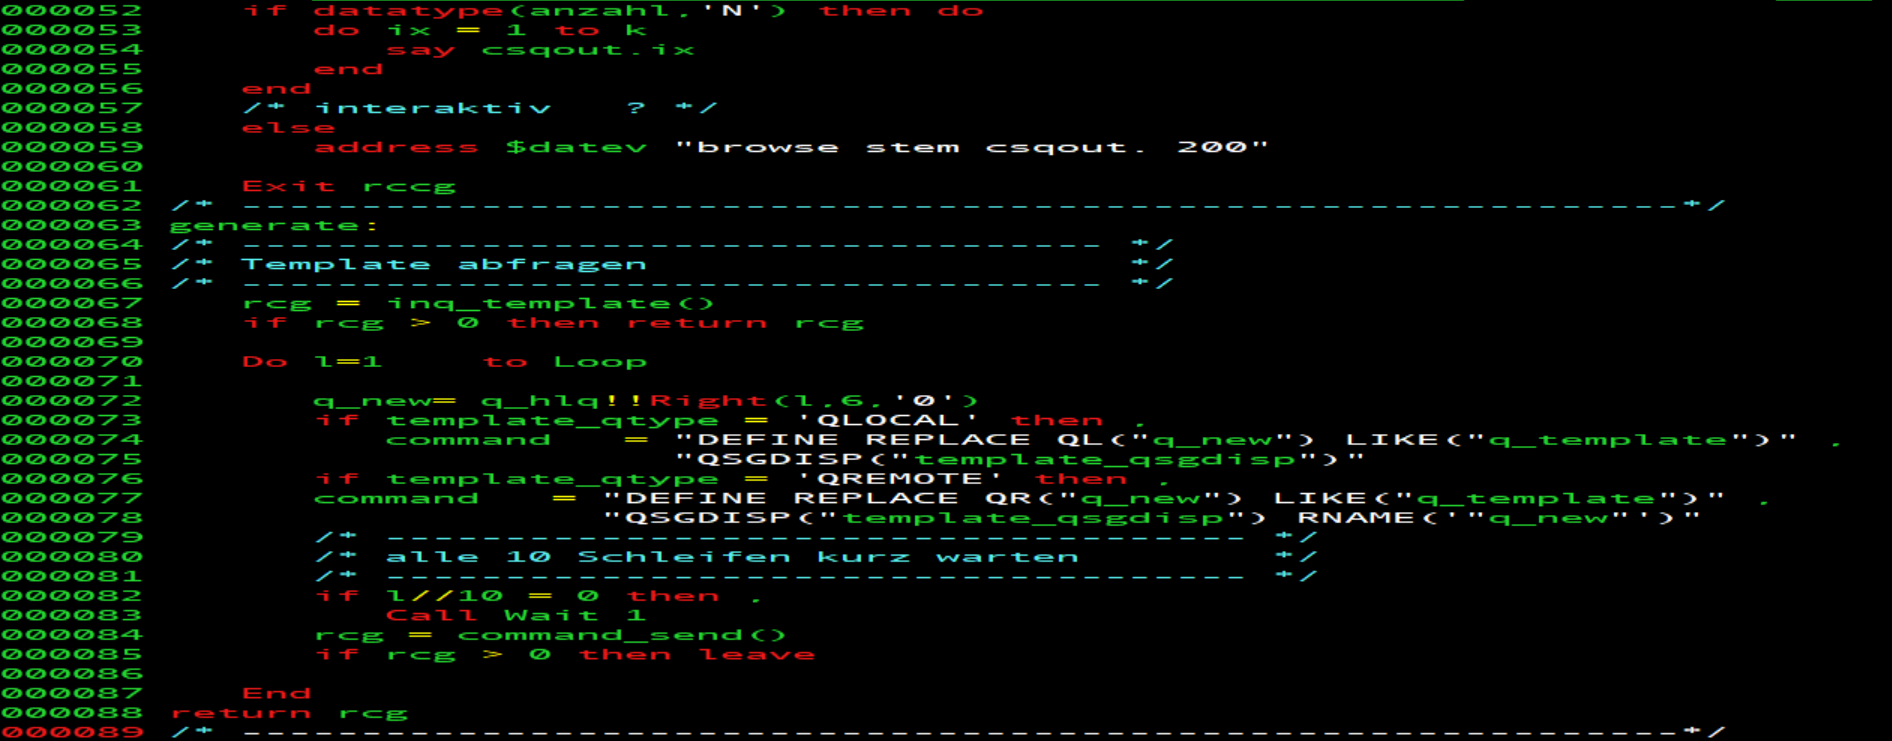
\includegraphics[width=\textwidth]{figures/rexxintso.png}
\caption{Auszug aus einem REXX Skript in der ISPF Oberfläche}
\label{fig:3270}
\end{figure}
Ein Meilenstein für die modernisierte z/OS Entwicklung bei DATEV war die Einführung von Git im Jahr 2018 auch für z/OS Sourcen. 
Dieses weit verbreitete Standard-Tool ist im z/OS Umfeld tatsächlich eine entscheidende Neuerung.
Dadurch wurde ein bis dato verwendetes eigenentwickeltes Tool für die Sourceverwaltung der z/OS Sourcen abgelöst.
Dieses stellte nur ein sehr einfaches Versionierungskonzept ohne aus Git bekannte Features wie Merge, Branch usw. bereit. 
Parallelentwicklung von verschiedenen Features war vorher mit viel Aufwand und Abstimmung möglich. 
Das Tooling wurde somit modernisiert, jedoch nicht der Entwicklungsprozess selbst.
Es teilen sich sehr viele Anwendungen die gleichen Entwicklungs-CICS/Db2/MQ Ressourcen.
Das heißt auch, dass eine Parallelentwicklung - trotz jetzt möglichen Git-Branches - an unterschiedlichen Features nur mit viel Abstimmungsaufwand und Absprachen innerhalb eines Entwicklungsteams, teilweise auch abteilungsübergreifend, möglich ist.
Werden Änderungen an bestehenden Ressourcen durchgeführt oder werden neue Systemumgebungen benötigt, entsteht weiterer Abstimmungsaufwand und weitere Absprachen.
Dadurch ist der aktuelle Prozess fehleranfällig und langsam.

Es bleibt die Frage, wie wird vor diesem Hintergrund mit den vielen Mainframebestandsanwendungen bei der DATEV e.G. in Zukunft umgegangen?
Die komplette Ablösung dieser Anwendungen durch cloud-native Lösungen ist eine Option, deren zeitlicher Rahmen und Machbarkeit aktuell nicht absehbar ist.\footnote{\ref{app:momappp} }
Für die Funktionsfähigkeit dieses Bestandsgeschäfts, das die Core-Business-Funktionalitäten der DATEV e.G. darstellt, muss also effiziente Weiterentwicklung und Wartung gewährleistet werden.
Auch im Falle einer geplanten Ablöse von Anwendungen muss je nach Strategie (z.B. \glqq Rewrite\grqq / \glqq Rearchitect\grqq)\footnote{(Kommentar, Strategiepatterns lt. Gartner, ich schick DIr enien Link)} das Alt-System parallel dazu über Jahre oder Jahrzehnte gepflegt und funktional aktuell gehalten werden.
Daraus folgt, dass aus Sicht der DATEV e.G. weiter in die IBM Mainframe Plattform investiert werden muss. 
Dies bedeutet Investitionen in die bereitgestellte Infrastruktur (Hardware, Betriebssysteme, Lizenzen), insbesondere aber auch Investitionen, die die oben genannten Anforderungen an Weiterentwicklung, Wartung und Entwicklungseffizienz sowie Effizienz im Betrieb adressieren.

\section{Ziel der Arbeit}\label{sec:ziel}
Es liegt also nahe, sich an den oben beschriebenen Prozessen zu cloud native Entwicklung zu orientieren. 
In diesem Zusammenhang läuft aktuell  bei DATEV e.G. ein Proof of Concept bezüglich automatisierter Builds von z/OS Anwendungen auf Basis von Jenkins basierten Pipelines. 
Dies ist auch die Voraussetzung für automatisierte Tests von z/OS Programmen im Rahmen des \glqq Continuous Integration, Continuous Deployment\grqq{} Ansatzes.
Was jedoch fehlt, sind \glqq Self Services\grqq{} für  Laufzeitumgebung und  Middleware.
Die dafür notwendige automatisierte Provisionierung einer z/OS Anwendungsumgebung, d.h Laufzeit, Middleware etc., ist aktuell noch weitgehend unerforscht. 
Hier sind die Prozesse bei DATEV und anderen Kunden oft noch proprietär, hoch spezialisiert,  manuell und nicht modernisiert. 
Gerade bei Mitarbeitern im Betrieb, die als Administratoren für die Middleware-Produkte arbeiten, sind die Bedenken groß, ob man diese Cloud-Vorgehensweise auf hochspezialisierte individuelle Komponenten wie CICS, DB2, IBM MQ anwenden kann, \glqq weil man so etwas bisher nicht vermisst hat\grqq\footnote{Marcel Amrein, IBM Senior Technical Sales Professional (MQ and CICS) (Quelle: Anhang \ref{app:ibm})}.
IBM bietet eine Lösung mit dem \glqq IBM Cloud Provisioning and Management for z/OS\grqq-Toolkit. 
Dies hat sich noch nicht flächendeckend durchgesetzt, aber \glqq Viele Kunden haben [...] im Moment Interesse, jedoch warten viele hier auf die ersten Erfahrungen von anderen\grqq\footnote{Tobias Leicher, IBM Senior IT Specialist for CICS and zAPI (Quelle: Anhang \ref{app:ibm})}.
Hier setzt diese Arbeit an und klärt folgende Fragen:

\begin{samepage}
\begin{itemize}
\item Ist es möglich, den Bereitstellungsprozess für z/OS Anwendung bei DATEV e.G. mit Hilfe des \glqq IBM Cloud Provisioning and Management for z/OS\grqq-Tools an cloud native Prozesse anzunähern?
\item Erzeugt die Nutzung von \glqq IBM Cloud Provisioning and Management for z/OS\grqq{} einen Mehrwert bei den Stakeholdern, also den Entwicklerteams und den Administratorenteams?
\end{itemize}
\end{samepage}

Um diese Fragen zu beantworten wird die Provisionierung einer z/OS Laufzeitumgebung für eine bestehende Anwendung untersucht.
Diese Anwendung sollte CICS als Anwendungsserver, eine Db2 Datenbank und IBM MQ als Messaginglösung nutzen, um für diese 3 Haupt-Technologien (Middleware-Komponenten) eine Aussage treffen zu können.
Die genaue Vorgehensweise wird im Kapitel \ref{ch:vorgehensweise} beschrieben.
